\chapter{The Monte Carlo Random Walk Process for Radiation Transport}
\label{ch:particle_transport}
In the previous chapter, the Monte Carlo random walk process was discussed in a 
very general mathematical sense. In this chapter, it will be shown how to apply
the general Monte Carlo random walk process to radiation transport 
problems. This will require the derivation of the PDFs that govern the random 
walk process from the transport equation. This derivation will be done in
some detail so that each step of the derivation is very clear. The same steps
that are shown in this chapter will then be followed in the next chapter
to derive the PDFs that govern the random walk process for adjoint radiation
transport. 

\section{The Integro-Differential Transport Equation}
\label{sec:int_diff_transport_eqn}
The equation that describes the average behavior of both photons and neutrons
in a medium is the transport equation:
\begin{equation}
  \begin{split}
    \frac{1}{v}&\frac{\partial \varphi(\vec{r},E,\hat{\Omega},t)}{\partial t} +
    \hat{\Omega} \cdot \vec{\bigtriangledown} \varphi(\vec{r},E,\hat{\Omega},t)
    + \Sigma_T(\vec{r},E) \varphi(\vec{r},E,\hat{\Omega},t) = \\
    & \quad S(\vec{r},E,\hat{\Omega},t) +
    \int\int \Sigma_T(\vec{r},E^{'} \to E,\hat{\Omega^{'}} \to \hat{\Omega})
    \varphi(\vec{r},E^{'},\hat{\Omega^{'}},t) dE^{'}d\hat{\Omega^{'}} 
  \end{split}
  \label{eq:integro_diff_boltzmann_eqn}
\end{equation}
where
\begin{align}
  \vec{r} & = \text{spacial coordinate} \nonumber \\
  E & = \text{energy} \nonumber \\
  \hat{\Omega} & = \text{flight direction} \nonumber \\
  t & = \text{time} \nonumber \\
  v & = \text{speed} \nonumber. \\
\end{align} 
The transport equation only characterizes the average or expected behavior of 
the radiation in a system. Therefore, the continuous function
$\varphi(\vec{r},E,\hat{\Omega},t)$ in equation 
\ref{eq:integro_diff_boltzmann_eqn} can be interpreted as the expected particle 
flux at $\vec{r}$ and time $t$ for particles with energy $E$ and direction
$\hat{\Omega}$ per unit energy per unit solid angle. The external particle 
source density is described by the function $S(\vec{r},E,\hat{\Omega},t)$. It 
can be interpreted as the probability per unit time that a particle of energy 
$E$ will appear at $\vec{r}$ per unit volume per unit energy per unit solid 
angle. The function $\Sigma_T(\vec{r},E)$ is the total macroscopic cross 
section at $\vec{r}$ for particles with energy $E$. It can be interpreted as the
probability of a particle interaction per unit distance of particle travel. The 
double differential collision cross section is represented by the function 
$\Sigma_T(\vec{r},E^{'} \to E,\hat{\Omega}^{'} \to \hat{\Omega})$, which can be 
interpreted as the total probability per unit distance per unit energy per unit 
solid angle at $\vec{r}$ for the transfer of a particle with energy $E^{'}$ and 
direction $\hat{\Omega}^{'}$ to the energy $E$ and direction $\hat{\Omega}$ as a
result of a collision. This double differential collision cross section can be 
expanded into the total macroscopic cross section and a total double 
differential transfer function. Also note that the total macroscopic cross 
section is just the sum of all partial macroscopic cross sections 
\citep{bell_nuclear_1979}: 
\begin{align}
  \Sigma_T(\vec{r},E^{'} \to E,\hat{\Omega}^{'} \to \hat{\Omega}) & =
  \Sigma_T(\vec{r},E^{'})
  f(\vec{r},E^{'} \to E,\hat{\Omega}^{'} \to \hat{\Omega}) \\
  & = \sum_i \Sigma_i(\vec{r},E^{'}) c_i(\vec{r},E^{'})
  f_i(\vec{r},E^{'} \to E,\hat{\Omega}^{'} \to \hat{\Omega}).
  \label{eq:expanded_diff_collision_cross_sec}
\end{align} 

Because the transport equation only takes into account average behavior, 
reactions that result in the emission of additional particles are handled 
implicitly. The double differential transfer function for each reaction
can therefore only describe the average outgoing energy and direction 
distribution for all particles emitted from the reaction. Some texts on neutron 
transport normalize the double differential transfer function for each reaction 
to the number of particles emitted from the reaction \citep{bell_nuclear_1979}. 
However, to facilitate eventual sampling from these distributions, they will 
instead be normalized to unity:
\begin{equation}
  \int\int f_i(\vec{r},E^{'} \to E,\hat{\Omega}^{'} \to \hat{\Omega})
  dEd\hat{\Omega} = 1
\end{equation}
The number of particles emitted from reaction $i$ will then be accounted for by 
the function $c_i(\vec{r},E^{'})$. For absorption reactions like the 
(n,$\gamma$) and (n,$\alpha$) neutron reactions and the photoelectric effect 
for photons, the function $c_i(\vec{r},E^{'})$ must be set equal to zero. For 
the elastic and inelastic scattering reactions of neutrons and gamma rays, the 
function $c_i(\vec{r},E^{'})$ will be set equal to unity. For the (n,2n) 
neutron reaction and the pair production photon reaction (neglecting charged 
particle creation), the function $c_i(\vec{r},E^{'})$ will be set equal to two. 
For fission reactions, the function $c_i(\vec{r},E^{'})$ will be set equal to 
the average number of neutrons produced by a fission caused by a neutron of 
energy $E^{'}$, $\nu(\vec{r},E^{'})$. Based on these definitions for the 
function $c_i(\vec{r},E^{'})$ the normalization for the total double 
differential transfer function can be determined: 
\begin{align}
  \int\int   \Sigma_T(\vec{r},E^{'})
  f(\vec{r},E^{'} \to E,\hat{\Omega}^{'} \to \hat{\Omega}) 
  dEd\hat{\Omega}
  & = \int\int \sum_i \Sigma_i(\vec{r},E^{'}) c_i(\vec{r},E^{'}) \nonumber \\
  & \qquad \quad \quad \cdot  
  f_i(\vec{r},E^{'} \to E,\hat{\Omega}^{'} \to \hat{\Omega}) 
  dEd\hat{\Omega} \nonumber \\
  \int\int f(\vec{r},E^{'} \to E,\hat{\Omega}^{'} \to \hat{\Omega}) 
  dEd\hat{\Omega} 
  & = \frac{\sum_i \Sigma_i(\vec{r},E^{'}) c_i(\vec{r},E^{'})}
             {\Sigma_T(\vec{r},E^{'})} \nonumber \\
  & = c(\vec{r},E^{'}).
\end{align}
The function $c(\vec{r},E^{'})$ is simply a cross section weighted average of
the $c_i(\vec{r},E^{'})$ functions for each reaction. It can be interpreted as
the mean number of particles (of the same type as the primary) emerging per 
collision at $\vec{r}$ given a particle of energy $E^{'}$.
  
While this consolidation of the double differential transfer function for each 
reaction into a total double differential transfer function is necessary in the 
context of the transport equation, it is not necessary in a Monte Carlo random 
walk process. In fact, the creation of a total double differential transfer 
function that adequately described the behavior of the particle is quite 
challenging. Instead, one must model each reaction type separately by using the 
double differential transfer function for an associated reaction. 

\section{The Transport equation in Integral Form}
The transport equation is often given in an integro-differential form, as seen 
in equation \ref{eq:integro_diff_boltzmann_eqn}. In order to use the Monte 
Carlo random walk process that was discussed in the previous chapter, the 
integro-differential form of the transport equation must be converted to a 
FIESK. Once it is in the appropriate form the PDFs that govern the random walk 
process for the radiation type of interest can be determined. Similar 
derivations to the one that will be shown can also be found in several 
references \citep{lewis_computational_1993, hoogenboom_adjoint_1977, irving_adjoint_1971, bell_nuclear_1979}.
 
In this report all problems discussed will be assumed to be steady state. 
Therefore, the time dependence of the transport equation, shown in equation 
\ref{eq:integro_diff_boltzmann_eqn}, will be ignored from here. To further 
simplify equation \ref{eq:integro_diff_boltzmann_eqn} the right hand side of 
the equation will be referred to simply as the emission density 
$\chi(\vec{r},E,\hat{\Omega})$:
\begin{equation}
    \chi(\vec{r},E,\hat{\Omega}) = S(\vec{r},E,\hat{\Omega}) +
    \int\int \Sigma_T(\vec{r},E^{'} \to E,\hat{\Omega}^{'} \to \hat{\Omega})
    \varphi(\vec{r},E^{'},\hat{\Omega}^{'}) dE^{'}d\hat{\Omega}^{'}.
  \label{eq:emission_density}
\end{equation}
The simplified transport equation then becomes
\begin{equation}
  \hat{\Omega} \cdot \vec{\bigtriangledown} \varphi(\vec{r},E,\hat{\Omega})
  + \Sigma_T(\vec{r},E) \varphi(\vec{r},E,\hat{\Omega}) =  
 \chi(\vec{r},E,\hat{\Omega}).
  \label{eq:reduced_transport_eqn}
\end{equation}

From the reduced transport equation, the method of characteristics will be 
used to transform it to its integral form. The characteristic for the transport 
equation is the line defined by the fixed point $\vec{r}$ and the direction 
$\hat{\Omega}$. This line can be parameterized by the variable $R$ resulting in 
the following equation:
\begin{equation}
  \vec{r}^{'} = \vec{r} - R\hat{\Omega}.
  \label{eq:characteristic}
\end{equation}
Using equation \ref{eq:characteristic} a directional derivative along the
characteristic can be determined:
\begin{align}
  \frac{d}{dR} & = \frac{dx^{'}}{dR}\frac{\partial}{\partial x} +
  \frac{dy^{'}}{dR}\frac{\partial}{\partial y} +
  \frac{dz^{'}}{dR}\frac{\partial}{\partial z} \nonumber \\
  & = -\Omega_x \frac{\partial}{\partial x} -
  \Omega_y \frac{\partial}{\partial y} -
  \Omega_z \frac{\partial}{\partial z} \nonumber \\
  & = -\hat{\Omega} \cdot \vec{\bigtriangledown}.
\end{align}
By using this directional derivative along the characteristic the transport 
equation can be reduced to a first order ordinary differential equation (ODE):
\begin{equation}
  -\frac{d}{dR}\varphi(\vec{r}^{'},E,\hat{\Omega}) + \Sigma_T(\vec{r}^{'},E)
  \varphi(\vec{r}^{'},E,\hat{\Omega}) =
  \chi(\vec{r}^{'},E,\hat{\Omega}).
  \label{eq:transport_ode}
\end{equation}
This ODE can be easily solved with the integrating factor
\begin{equation*}
\exp{\left[-\int_0^R \Sigma_T(\vec{r}-R^{'}\hat{\Omega},E)dR^{'} \right]},
\end{equation*}
as will be shown. 

First, the left two terms of equation \ref{eq:transport_ode} can be combined 
into a single term using the integrating factor:
\begin{align}
  -\frac{d}{dR}\bigg[\varphi(\vec{r}^{'},E,\hat{\Omega})
      \exp{\left[-\int_0^R \Sigma_T(\vec{r}-R^{'}\hat{\Omega},E)dR^{'}\right]
      \bigg]} & = \nonumber \\
  \chi(\vec{r}^{'},E,\hat{\Omega})
  &\exp{\left[-\int_0^R \Sigma_T(\vec{r}-R^{'}\hat{\Omega},E)dR^{'} \right]}
  \nonumber
\end{align}
Next, the derivative along the characteristic can be eliminated by integrating 
from zero to infinity:
\begin{align}
    -\varphi(\vec{r} - R\hat{\Omega},E,\hat{\Omega})
    \exp{\left[-\int_0^R \Sigma_T(\vec{r}-R^{'}\hat{\Omega},E)dR^{'}\right]}
    \bigg|_0^{\infty} & = \nonumber \\
    \int_0^{\infty} 
    \chi(\vec{r} - R\hat{\Omega},E,\hat{\Omega})
    &\exp{\left[-\int_0^R \Sigma_T(\vec{r}-R^{'}\hat{\Omega},E)dR^{'} \right]} dR.
    \nonumber
\end{align}
If the flux is assumed to go to zero as R goes to infinity, the integral 
transport equation is obtained:
\begin{equation}
    \varphi(\vec{r},E,\hat{\Omega}) = 
    \int_0^{\infty} \chi(\vec{r} - R\hat{\Omega},E,\hat{\Omega})
    \exp{\left[-\int_0^R \Sigma_T(\vec{r}-R^{'}\hat{\Omega},E)dR^{'} \right]} dR.
  \label{eq:line_integral_transport_eqn}
\end{equation}

It is often more convenient to represent the integral transport equation as an 
integral over all space instead of a line integral. To convert equation 
\ref{eq:line_integral_transport_eqn} to a volume integral, note that
\begin{align} 
  R & = |\vec{r} - \vec{r}^{'}| \text{,} \nonumber \\
  \hat{\Omega} & = \frac{\vec{r} - \vec{r}^{'}}{|\vec{r} - \vec{r}^{'}|} 
  \text{ and} \nonumber \\
  dV^{'} & = R^2dRd\hat{\Omega}.
\end{align}
With the above definitions, the integral transport equation becomes
\begin{equation*}
  \varphi(\vec{r},E,\hat{\Omega}) = 
  \int \chi(\vec{r}^{'},E,\hat{\Omega})
  \exp{\Big[-\int_0^{|\vec{r} - \vec{r}^{'}|} 
      \Sigma_T(\vec{r}-R^{'}\hat{\Omega},E)dR^{'} \Big]} \\
  \frac{\delta \left(\hat{\Omega} - \left[\frac{\vec{r} - \vec{r}^{'}}
      {|\vec{r} - \vec{r}^{'}|}\right]\right)}
        {|\vec{r} - \vec{r}^{'}|^2} dV^{'}.
\end{equation*}

To further simplify the integral transport equation, one more function will be 
introduced:
\begin{equation}
  \tau(\vec{r}^{'},\vec{r},E,\hat{\Omega}) = 
  \exp{\left[-\int_0^{|\vec{r} - \vec{r}^{'}|} 
              \Sigma_T(\vec{r}-R^{'}\hat{\Omega},E)dR^{'} \right]}
    \frac{\delta \left(\Omega - \left[\frac{\vec{r} - \vec{r}^{'}}
        {|\vec{r} - \vec{r}^{'}|}\right]\right)} 
    {|\vec{r} - \vec{r}^{'}|^2}.
  \label{eq:unnormalized_transport_kernel}
\end{equation}
The simplified integral transport equation is now simply
\begin{equation}
  \varphi(\vec{r},E,\hat{\Omega}) =
  \int \chi(\vec{r}^{'},E,\hat{\Omega})
  \tau(\vec{r}^{'},\vec{r},E,\hat{\Omega}) dV^{'}.
  \label{eq:volume_integral_transport_eqn}
\end{equation}

With the transport equation now in an integral form, only minor manipulations
are needed in order to turn it into a FIESK.

\section{The Flux FIESK}
\label{sec:flux_fiesk}
To derive the flux FIESK, the emission density defined in equation 
\ref{eq:emission_density} will be substituted back into the integral
transport equation shown in equation \ref{eq:volume_integral_transport_eqn}:
\begin{align}
  \varphi(\vec{r},E,\hat{\Omega}) & = \int \left[
    S(\vec{r}^{'},E,\hat{\Omega}) + 
    \int\int \Sigma_T(\vec{r}^{'},E^{'} \to E, \hat{\Omega}^{'} \to \hat{\Omega})
    \varphi(\vec{r}^{'},E^{'},\hat{\Omega}^{'})dE^{'}d\hat{\Omega}^{'} \right] 
  \nonumber \\
    & \qquad \cdot \tau(\vec{r}^{'},\vec{r},E,\hat{\Omega}) dV^{'}
  \nonumber \\
  \varphi(\vec{r},E,\hat{\Omega}) & =\int S(\vec{r}^{'},E,\hat{\Omega})
  \tau(\vec{r}^{'},\vec{r},E,\hat{\Omega}) dV^{'} + \nonumber \\
  & \quad \int\int\int \tau(\vec{r}^{'},\vec{r},E,\hat{\Omega})
  \Sigma_T(\vec{r}^{'},E^{'} \to E, \hat{\Omega}^{'} \to \hat{\Omega})
  \varphi(\vec{r}^{'},E^{'},\hat{\Omega}^{'}) dE^{'} d\hat{\Omega}^{'} dV^{'}.
  \label{eq:flux_integral_equation}
\end{align}

Since equation \ref{eq:flux_integral_equation} is a FIESK that describes the
flux, a random walk process can be created to simulate the flux. The source PDF 
will be created first (using the same notation from the previous chapter):
\begin{equation}
  p^1(\vec{r},E,\hat{\Omega}) = \frac{\int S(\vec{r}^{'},E,\hat{\Omega})
    \tau(\vec{r}^{'},\vec{r},E,\hat{\Omega}) dV^{'}}{\int\int S(\vec{r}^{'},E,\hat{\Omega})
    \tau(\vec{r}^{'},\vec{r},E,\hat{\Omega}) dV^{'} dV dE d\hat{\Omega}}.
\end{equation}
The state transition PDF can be broken into two parts; one part will govern the
movement of the particle through space and the other part will govern the 
movement of the particle through energy and direction: 
\begin{align}
  p(y \to x) & =
  p(\vec{r}^{'} \to \vec{r}, E^{'} \to E, \hat{\Omega}^{'} \to \hat{\Omega})
  \nonumber \\
  & = p(\vec{r}^{'} \to \vec{r}\quad| E,\hat{\Omega})
  p(E^{'} \to E, \hat{\Omega}^{'} \to \hat{\Omega}\quad|\vec{r}^{'}).
\end{align} 

The PDF that governs the movement through space is simply the function 
$\tau(\vec{r}^{'},\vec{r},E,\hat{\Omega})$ defined in equation 
\ref{eq:unnormalized_transport_kernel} normalized to unity: 
\begin{align}
  p(\vec{r}^{'} \to \vec{r} \quad | E,\hat{\Omega}) & =
  \frac{\tau(\vec{r}^{'},\vec{r},E,\hat{\Omega})}
       {w_1(\vec{r}^{'},E,\hat{\Omega})},  \\
  \text{ wh}&\text{ere} \nonumber \\
  w_1(\vec{r}^{'},E,\hat{\Omega}) & = \int \tau(\vec{r}^{'},\vec{r},E,\hat{\Omega}) dV.
\end{align}

The random walk process that would correspond to the flux FIESK has many
disadvantages. First, during the random walk process the weight of the 
particle after every collision will be multiplied by the factor $w_1$. 
Unfortunately, this factor is not bounded to the interval $(0,1)$ and will 
likely increase the variance of the estimator used \citep{spanier_monte_1969}. 
Another disadvantage of this random walk process comes about from the 
conditional state transition PDF 
$p(\vec{r}^{'} \to \vec{r}\quad| E,\hat{\Omega})$. Because this PDF does not 
contain the factor $\Sigma_T(\vec{r},E)$, it is possible to sample an event 
position in a vacuum. This peculiar property is due to the fact that the flux 
does not go to zero in a vacuum. The final disadvantage is that sampling from
the source would be very challenging given that the source is defined as
an integral which is difficult to evaluate in general.

The Monte Carlo random walk process for estimating the flux directly is not 
ideal and in practice is rarely done. An event density should have a preferable 
random walk process because at the very least, the event density goes to zero 
in a vacuum. 

\section{The Emission Density FIESK}
A FIESK will now be constructed for the emission density. To construct the
flux FIESK, the emission density given in equation \ref{eq:emission_density} was
substituted into the integral transport equation shown in equation 
\ref{eq:volume_integral_transport_eqn}. To construct the emission density FIESK,
the opposite will be done. 
\begin{align}
    \chi(\vec{r},E,\hat{\Omega}) & = S(\vec{r},E,\hat{\Omega}) +
    \int\int \Sigma_T(\vec{r},E^{'} \to E, \hat{\Omega}^{'} \to \hat{\Omega})
    \int \chi(\vec{r}^{'},E',\hat{\Omega}^{'})
    \tau(\vec{r}^{'},\vec{r},E^{'},\hat{\Omega}^{'})dV^{'}dE^{'}d\hat{\Omega}^{'} 
    \nonumber \\
    & = S(\vec{r},E,\hat{\Omega}) + \int\int\int
    \frac{\Sigma_T(\vec{r},E^{'} \to E, \hat{\Omega}^{'} \to \hat{\Omega})}
    {\Sigma_T(\vec{r},E^{'})} \Sigma_T(\vec{r},E^{'}) 
    \tau(\vec{r}^{'},\vec{r},E^{'},\hat{\Omega}^{'}) \nonumber \\
    & \qquad \qquad \qquad \qquad \qquad \cdot 
    \chi(\vec{r}^{'},E',\hat{\Omega}^{'}) dV^{'}dE^{'}d\hat{\Omega}^{'} \nonumber
\end{align}

Two kernels must now be introduced to simplify the emission density FIESK. The
first will be called the collision kernel and is defined as 
\begin{align}
  C(\vec{r},E^{'} \to E,\hat{\Omega}^{'} \to \hat{\Omega}) & = 
  \frac{\Sigma_T(\vec{r},E^{'} \to E,\hat{\Omega}^{'} \to \hat{\Omega})}
       {\Sigma_T(\vec{r},E^{'})} \nonumber \\
  & = f(\vec{r},E^{'} \to E,\hat{\Omega}^{'} \to \hat{\Omega})
\end{align}
Note that the collision kernel is simply the total double differential transfer 
function that was discussed in section \ref{sec:int_diff_transport_eqn}.
The second kernel will be called the transport kernel and is defined as
\begin{align}
  T(\vec{r}^{'} \to \vec{r},E,\hat{\Omega}) & = \Sigma_T(\vec{r},E)
  \tau(\vec{r}^{'},\vec{r},E,\hat{\Omega}) \nonumber \\
  & = \Sigma_T(\vec{r},E)
  \exp{\left[-\int_0^{|\vec{r} - \vec{r}^{'}|} 
    \Sigma_T(\vec{r}-R^{'}\hat{\Omega},E)dR^{'} \right]} 
  \frac{\delta \left(\hat{\Omega} - \left[\frac{\vec{r} - \vec{r}^{'}}
      {|\vec{r} - \vec{r}^{'}|}\right]\right)}
       {|\vec{r} - \vec{r}^{'}|^2}.
  \label{eq:transport_kernel}
\end{align}
Note that the quantity $T(\vec{r}^{'} \to \vec{r},E,\hat{\Omega})dV$ can be 
interpreted as the probability that a particle at $\vec{r}^{'}$ with energy $E$ 
and direction $\hat{\Omega}$ will have its next collision in volume element $dV$
at $\vec{r}$.
 
Using the above kernels, the simplified emission density FIESK becomes
\begin{align}
\chi(\vec{r},E,\hat{\Omega}) & = S(\vec{r},E,\hat{\Omega}) +
    \int\int\int C(\vec{r},E^{'} \to E,\hat{\Omega}^{'} \to \hat{\Omega})
    T(\vec{r}^{'} \to \vec{r},E^{'},\hat{\Omega}^{'}) \nonumber \\
    & \qquad \qquad \qquad \qquad \qquad \cdot 
    \chi(\vec{r}^{'},E',\hat{\Omega}^{'}) dV^{'}dE^{'}d\hat{\Omega}^{'}.
    \label{eq:emission_density_integral_eqn}
\end{align}

The state transition kernel for the emission density FIESK is simply 
\begin{align}
  K(y \to x) & = K(\vec{r}^{'} \to \vec{r}, E^{'} \to E, 
  \hat{\Omega}^{'} \to \hat{\Omega}) \nonumber \\
  & = C(\vec{r},E^{'} \to E,\hat{\Omega}^{'} \to \hat{\Omega})
  T(\vec{r}^{'} \to \vec{r},E^{'},\hat{\Omega}^{'}).
\end{align}

\section{The Collision Density FIESK}
Up to this point, only the flux and the emission density have been discussed.
However, there is another quantity that can be very useful: the collision 
density. It is related to the flux and the emission density by the following 
equations:
\begin{align}
  \psi(\vec{r},E,\hat{\Omega}) & = \Sigma_T(\vec{r},E)
  \varphi(\vec{r},E,\hat{\Omega}) \\
  & = \int T(\vec{r}^{'} \to \vec{r},E,\hat{\Omega})
  \chi(\vec{r}^{'},E,\hat{\Omega})dV^{'}.
  \label{eq:collision_emission_relation}
\end{align}
The kernel $T(\vec{r}^{'} \to \vec{r},E,\hat{\Omega})$ is the transport kernel
that was defined in equation \ref{eq:transport_kernel}. Whereas the emission 
density is the expected density of particles exiting a collision or the source, 
the collision density is the expected density of particles entering a collision.

To construct the collision density FIESK, equation 
\ref{eq:collision_emission_relation} and the emission density FIESK given in
equation \ref{eq:emission_density_integral_eqn} will be used:
\begin{align}
  \psi(\vec{r},E,\hat{\Omega}) & = \int S(\vec{r}^{'},E,\hat{\Omega})
  T(\vec{r}^{'} \to \vec{r},E,\hat{\Omega}) dV^{'} + \nonumber \\
  & \quad \int\int\int
  T(\vec{r}^{'} \to \vec{r},E,\hat{\Omega})  
  C(\vec{r}^{'},E^{'} \to E,\hat{\Omega}^{'} \to \hat{\Omega}) 
  \psi(\vec{r}^{'},E^{'},\hat{\Omega}^{'}) dE^{'}d\hat{\Omega}^{'}dV^{'}.
  \label{eq:collision_density_integral_eqn}
\end{align}
Notice that the source term for the collision density FIESK is the first
collided source.

The state transition kernel for the collision density FIESK is simply
\begin{align}
  L(y \to x) & = 
  L(\vec{r}^{'} \to \vec{r},E^{'} \to E,\hat{\Omega}^{'} \to \hat{\Omega}) 
  \nonumber \\
  & = T(\vec{r}^{'} \to \vec{r},E,\hat{\Omega})
  C(\vec{r}^{'},E^{'} \to E,\hat{\Omega}^{'} \to \hat{\Omega}).
\end{align}

\section{Emission and Collision Density State Transition Kernel Properties}
Before the PDFs that govern the random walk process for the emission and
collision densities are derived, the transport and collision kernels must be 
investigated a bit further. First, note that for an infinite medium the 
transport kernel is normalized:
\begin{align}
  \int T(\vec{r}^{'} \to \vec{r},E,\hat{\Omega})dV & =
    \int \Sigma_T(\vec{r},E)
    \cdot exp\Big[-\int_0^{|\vec{r} - \vec{r}^{'}|} 
      \Sigma_T(\vec{r}-R^{'}\hat{\Omega},E)dR^{'} \Big] 
    \frac{\delta \left(\Omega - \left[\frac{\vec{r} - \vec{r}^{'}}
        {|\vec{r} - \vec{r}^{'}|}\right]\right)}
    {|\vec{r} - \vec{r}^{'}|^2} dV \nonumber \\
  & = \int_0^{\infty} \Sigma_T(\vec{r}^{'}+R\hat{\Omega},E)
  \cdot exp\left[-\int_0^R \Sigma_T(\vec{r}^{'}+R^{''}\hat{\Omega},E)
    dR^{''} \right] dR \nonumber \\
  & = -\int_0^{\infty} \frac{d}{dR} exp\left[-\int_0^R 
    \Sigma_T(\vec{r}^{'}+R^{''}\hat{\Omega},E) dR^{''} \right] dR 
  \nonumber \\
  & = 1. \nonumber
\end{align}
However, if the domain of interest in a problem is finite, the transport kernel 
will no longer be normalized. Fortunately, this is taken care of by terminating 
random walks that exit the domain of interest, which is equivalent to 
surrounding the domain of interest with a purely absorbing medium of infinite 
extent \citep{irving_adjoint_1971}.

The collision kernel, being equal to the total double differential transfer 
probability, has the following property:
\begin{equation}
  \int\int C(\vec{r},E^{'} \to E,\hat{\Omega}^{'} \to \hat{\Omega}) 
  dEd\hat{\Omega} = c(\vec{r},E^{'}),
  \label{eq:collision_op_prop_gen}
\end{equation}
where $c(\vec{r},E^{'})$ is the mean number of particles emitted per collision
at $\vec{r}$ given a particle of energy $E^{'}$. In regions where no 
multiplying reactions occur, the collision kernel has the following, more 
familiar property:
\begin{align}
  \int\int C(\vec{r},E^{'} \to E,\hat{\Omega}^{'} \to \hat{\Omega}) 
  dEd\hat{\Omega} & = \frac{\Sigma_s(\vec{r},E^{'})}{\Sigma_T(\vec{r},E^{'})}
  \label{eq:collision_op_prop} \\
  & = P_{NA}(\vec{r},E^{'}). \nonumber 
\end{align}
The macroscopic cross section $\Sigma_s(\vec{r},E^{'})$ is the total macroscopic
scattering cross section. The ratio of the total macroscopic scattering cross
section and the total macroscopic cross section is often referred to as the 
non-absorption or survival probability, $P_{NA}(\vec{r},E)$. 

Based on these properties of the transport and collision kernels, the emission 
density state transition kernel normalization can be determined. If multiplying
reactions are possible in a region, the normalization is the following:
\begin{align}
  \int K(y \to x) dx & = \int\int\int 
  C(\vec{r},E^{'} \to E,\hat{\Omega}^{'} \to \hat{\Omega})
  T(\vec{r}^{'} \to \vec{r},E^{'},\hat{\Omega}^{'}) dE d\hat{\Omega} dV 
  \nonumber \\
  & = \int c(\vec{r},E^{'}) T(\vec{r}^{'} \to \vec{r},E^{'},\hat{\Omega}^{'})
  dV \nonumber \\
  & = \bar{c}(\vec{r}^{'},E^{'}).
\end{align}
The normalization function $\bar{c}(\vec{r}^{'},E^{'})$ can be interpreted as an 
average of the mean number of particles emerging per collision along the line 
from $\vec{r}^{'}$ to $\vec{r}$ given a particle of energy $E^{'}$. If 
multiplying reactions are not possible in a region, the normalization is instead
\begin{align}
  \int K(y \to x) dx & = \int\int\int 
  C(\vec{r},E^{'} \to E,\hat{\Omega}^{'} \to \hat{\Omega})
  T(\vec{r}^{'} \to \vec{r},E^{'},\hat{\Omega}^{'}) dE d\hat{\Omega} dV 
  \nonumber \\
  & = \int P_{NA}(\vec{r},E^{'}) T(\vec{r}^{'} \to \vec{r},E^{'},\hat{\Omega}^{'})
  dV \nonumber \\
  & = \overline{P}_{NA}(\vec{r}^{'},E^{'}).
\end{align}
The normalization function $\overline{P}_{NA}(\vec{r}^{'},E^{'})$ can be 
interpreted as the average survival probability along the line from 
$\vec{r}^{'}$ to $\vec{r}$ given a particle of energy $E^{'}$.

The collision density state transition kernel normalization can also be 
determined with the properties of the transport and collision kernels that 
were discussed. If multiplying reactions are possible in a region, the 
normalization is 
\begin{align}
  \int L(y \to x) dx & = \int\int\int
  T(\vec{r}^{'} \to \vec{r},E,\hat{\Omega})
  C(\vec{r}^{'},E^{'} \to E,\hat{\Omega}^{'} \to \hat{\Omega}) dV dE d\hat{\Omega}
  \nonumber \\
  & = \int\int 
  C(\vec{r}^{'},E^{'} \to E,\hat{\Omega}^{'} \to \hat{\Omega}) dE d\hat{\Omega} 
  \nonumber \\
  & = c(\vec{r}^{'},E^{'}).
\end{align}
In regions where multiplying reactions are not possible, the normalization is
instead 
\begin{align}
  \int L(y \to x) dx & = \int\int\int
  T(\vec{r}^{'} \to \vec{r},E,\hat{\Omega})
  C(\vec{r}^{'},E^{'} \to E,\hat{\Omega}^{'} \to \hat{\Omega}) dV dE d\hat{\Omega}
  \nonumber \\
  & = \int\int 
  C(\vec{r}^{'},E^{'} \to E,\hat{\Omega}^{'} \to \hat{\Omega}) dE d\hat{\Omega} 
  \nonumber \\
  & = P_{NA}(\vec{r}^{'},E^{'}).
\end{align}

The properties of the two state transition kernels are summarized below:
\begin{enumerate}
  \item $K(y \to x) > 0$ \\
    $L(y \to x) > 0$ \\ \\
    and
  \item $\int K(y \to x)dx = \bar{c}(y) >= \overline{P}_{NA}(y)$ \\
    $\int L(y \to x)dx = c(y) >= P_{NA}(y)$.
\end{enumerate}

In section \ref{sec:mc_random_walk_process}, where the necessary properties
of the random walk PDFs where enumerated, it was stated that the state
transition PDF integrated over final states must be equal to the survival 
probability in the initial state:
\begin{equation*}
  \int_{\Gamma}p(y \to x)dx = q(y) = 1-p(y)
\end{equation*}
The state transition kernel for the emission density and the collision density
will only have this property when multiplying reactions aren't possible. When
multiplying reactions are possible, the emission density state transition 
kernel will have to be multiplied by the factor
\begin{equation*}
  \frac{\overline{P}_{NA}(y)}{\bar{c}(y)},
\end{equation*}
and the collision density state transition kernel will have to be multiplied
by the factor
\begin{equation*}
  \frac{P_{NA}(y)}{c(y)}.
\end{equation*}
Due to these factors, it would appear that conducting an analogue random walk 
process for radiation transport without using weights is impossible in a system 
where multiplying reactions are possible. This is indeed true if particle 
multiplication is handled implicitly. However, if particle multiplication is 
handled explicitly, with separate random walks conducted for each additional 
particle emitted, an analogue random walk process can be conducted without 
using weights. To handle particle multiplication explicitly, the collision 
kernel must be expanded into its constituent parts, which will be shown in the 
next section.

\section{Expansion of the Collision Kernel}
As mentioned in the previous sections, to treat particle multiplication
explicitly, the collision kernel must be expanded:
\begin{align}
  C(\vec{r},E^{'} \to E, \hat{\Omega}^{'} \to \hat{\Omega}) & =
  \frac{\Sigma_T(\vec{r},E^{'} \to E,\hat{\Omega}^{'} \to \hat{\Omega})}
       {\Sigma_T(\vec{r},E^{'})} \nonumber \\
  & = f(\vec{r},E^{'} \to E,\hat{\Omega}^{'} \to \hat{\Omega}) \nonumber \\
  & = \sum_j \frac{\Sigma_j(\vec{r},E^{'})c_i(\vec{r},E^{'})
            f_i(\vec{r},E^{'} \to E,\hat{\Omega}^{'} \to \hat{\Omega})}
           {\Sigma_T(\vec{r},E^{'})} \nonumber \\
  & = \sum_A \frac{\Sigma_A(\vec{r},E^{'})}{\Sigma_T(\vec{r},E^{'})}
      \sum_j \frac{\sigma_{A,j}(E^{'})}{\sigma_A(E^{'})} c_{A,j}(E^{'})
      p_{A,j}(E^{'} \to E,\hat{\Omega}^{'} \to \hat{\Omega}) \nonumber \\
  & = \sum_A p_A(\vec{r},E^{'}) \sum_j p_{A,j}(E^{'}) 
      \sum_{k=1}^2 p_{A,j,k}(E^{'}) \nonumber \\
  & \qquad \qquad \qquad \qquad \qquad \quad
      \cdot \sum_{l=1}^{x_k} 
      p_{A,j,l}(E^{'} \to E,\hat{\Omega}^{'} \to \hat{\Omega}).
  \label{eq:fully_expanded_collision_kernel}
\end{align}
In this expansion, the subscript $A$ denotes a particular nuclide or element, 
the subscript $j$ denotes a particular type of reaction and the subscript $l$ 
denotes a particular emitted particle. The function 
$p_{A,j,l}(E^{'} \to E,\hat{\Omega}^{'} \to \hat{\Omega})$ is the double
differential transfer probability for the initial particle and emitted
particle l given a collision of type j on nuclide or element A. This transfer 
probability is normalized to unity. Since it is desired to conduct 
separate random walks for each emitted particle, only an integer number of 
particles can be emitted from a collision\footnote{The average number of 
particles emitted from fission will normally be a non-integer value}. The 
probabilities $p_{A,j,k}(E^{'})$ restrict the number of particles emitted to 
integer values. They are defined as follows along with the corresponding value 
of $x_k$:
\begin{align}
  p_{A,j,1} & =
  \begin{cases}
    \lceil c_{A,j}(E^{'}) \rceil - c_{A,j}(E^{'}) & \text{ if } c_{A,j}(E^{'})
    \text{ not an integer} \\
    1 & \text{ otherwise}
  \end{cases} \\
  p_{A,j,2} & = 1 - p_{A,j,1}
\end{align}
and
\begin{align}
  x_1 & = 
  \begin{cases}
    \lfloor c_{A,j}(E^{'}) \rfloor & \text{ if } c_{A,j}(E^{'})
    \text{ not an integer} \\
    c_{A,j}(E^{'}) & \text{ otherwise}
  \end{cases} \\
  x_2 & = \lceil c_{A,j}(E^{'}) \rceil.
\end{align}
The expected value of the number of emitted particles, based on these 
probabilities and corresponding number of emitted particles, is $c_{A,j}(E^{'})$
as required by the definition of the collision kernel.

By sampling from the collision kernel in its expanded form, particle
multiplication will be treated explicitly. In this process of sampling from
the expanded collision kernel one first samples the nuclide or element hit from 
the discrete PDF 
\begin{align}
  p(A|\vec{r},E^{'}) & = \sum_A p_A(\vec{r},E^{'}) \nonumber \\
  & = \sum_A \frac{\Sigma_A(\vec{r},E^{'})}{\Sigma_T(\vec{r},E^{'})}.
\end{align}
With the nuclide or element $A$ selected, the reaction type is sampled from the 
discrete PDF 
\begin{align}
  p(j|A,E^{'}) & = \sum_j p_{A,j}(E^{'}) \nonumber \\
  & = \sum_j \frac{\sigma_{A,j}(E^{'})}{\sigma_A(E^{'})} 
\end{align}
The number of particles emitted from the collision is then sampled from the 
discrete PDF
\begin{equation}
  p(x_k|E^{'}) = \sum_k p_{A,j,k}(E^{'}).
\end{equation}
Finally, for each emitted particle $l$, the outgoing energy and direction is 
sampled from the transfer probability 
$p_{A,j,l}(E^{'} \to E,\hat{\Omega}^{'} \to \hat{\Omega})$. 

In the sampling of the reaction type, if an absorption reaction is chosen, the 
random walk for the current particle ends. Therefore, at every collision, a 
random walk will end with probability 
\begin{equation*}
  \frac{\Sigma_A(\vec{r},E)}{\Sigma_T(\vec{r},E)}.
\end{equation*} 
This behavior mimics the behavior that was described in the random walk process 
from the previous chapter. Instead of separately sampling whether a random walk 
ends, it is now incorporated into the sampling of a new particle state.

\section{The Emission and Collision Density Random Walk PDFs}
With the state transition kernels $K(y \to x)$ and $L(y \to x)$ fully 
characterized, the Monte Carlo random walk process for radiation transport can 
be completely specified: 
\begin{align}
  \chi(x)\text{ Random Walk (implicit mult.):}&
  \begin{cases}
    p^1(x) & = \frac{S(x)}{\int_{\Gamma} S(x)dx} \\
    p(y \to x) &  = \frac{\overline{P}_{NA}(y)}{\bar{c}(y)}K(y \to x) \\
    p(x) & = 1 - \overline{P}_{NA}(x),
  \end{cases} \\
  \psi(x)\text{ Random Walk (implicit mult.):}&
  \begin{cases}
    p^1(x) & = \frac{S_c(x)}{\int_{\Gamma} S_c(x)dx} \\
    p(y \to x) & = \frac{P_{NA}(y)}{c(y)}L(y \to x) \\
    p(x) & = 1 - P_{NA}(x)
  \end{cases} \\
  \text{ and} \nonumber \\
  \nonumber \\
  \chi(x)\text{ Random Walk (explicit mult.):} &
  \begin{cases}
    p^1(x) & = \frac{S(x)}{\int_{\Gamma} S(x)dx} \\
    p(y \to x) &  = K(y \to x) \\
    p(x) & = 1 - \overline{P}_{NA}(x),
  \end{cases}
  \label{eq:mc_random_walk_emission_dens} \\
  \psi(x)\text{ Random Walk (explicit mult.):} &
  \begin{cases}
    p^1(x) & = \frac{S_c(x)}{\int_{\Gamma} S_c(x)dx} \\
    p(y \to x) & = L(y \to x) \\
    p(x) & = 1 - P_{NA}(x).
  \end{cases}
  \label{eq:mc_random_walk_collision_dens}
\end{align}
Note that the function $S_c(x)$ is simply the first collided source, which was
shown in equation \ref{eq:collision_density_integral_eqn}. The first set of 
processes is for treating multiplication implicitly\footnote{It must be noted 
that the random walk procedures that treat multiplication implicitly will never 
be used. This is because they rely on the total transfer probability, which is 
challenging to obtain and even more challenging to sample from directly. 
However, they are shown to provide continuity between this chapter and the 
previous chapter.}. The second set is for treating multiplication explicitly 
using the procedure outlined in the previous section. In the second set of 
processes, the termination probabilities aren't sampled directly. Instead, a 
random walk can potentially be terminated when sampling from $p(y \to x)$.

While it might appear from the above PDFs that the random walk processes for
the emission and collision density are completely different, because the kernels
$K(y \to x)$ and $L(y \to x)$ only differ in the ordering of the collision and 
transport kernels and because of the relationship between the emission density 
and the collision density, both can be estimated during the same random walk 
process. Figure \ref{fig:combined_random_walk_process} illustrates the new 
combined random walk process. In this new process, particles always start in 
the true source and not the first collided source, which is advantageous 
because the first collided source would be challenging to 
evaluate in general. The emission density will always be estimated right after 
a collision (or birth) and the collision density will always be estimated right 
before a collision. 
\begin{figure}[t!]
  \begin{center}
    \scalebox{0.75}{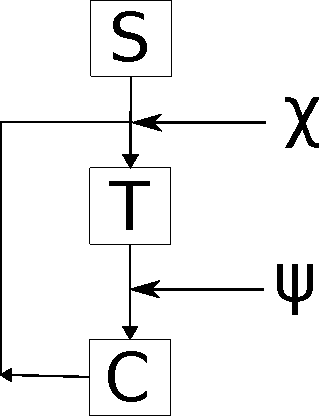
\includegraphics{chapters/random_walk_process_derivation/random_walk_process.pdf}}
    \end{center}
  \caption{\textbf{Monte Carlo random walk procedure for radiation.}
    \textit{A particle state is first sampled from the source distribution. The
      next collision point is sampled from the transport kernel T. Finally,
      the new particle energy and direction is sampled from the collision
      kernel, assuming that an absorption reaction wasn't sampled. If an
      absorption reaction was sampled, the random walk ends. Otherwise, the
      process continues. This procedure allows both the emission density and 
      the collision density to be estimated.}}
  \label{fig:combined_random_walk_process}
\end{figure}

A common modification to the previous analogue random walk processes is to 
ignore absorption and instead use weights to account for the absorption 
probability. This modification results in the following non-analogue
random walk processes. 
\begin{align}
  \chi(x)\text{ Random Walk (implicit mult.):}&
  \begin{cases}
    p^1(x) & = \frac{S(x)}{\int_{\Gamma} S(x)dx} \\
    p(y \to x) &  = \frac{K(y \to x)}{\bar{c}(y)} \\
    p(x) & = 0
  \end{cases} \\
  \psi(x)\text{ Random Walk (implicit mult.):}&
  \begin{cases}
    p^1(x) & = \frac{S_c(x)}{\int_{\Gamma} S_c(x)dx} \\
    p(y \to x) & = \frac{L(y \to x) }{c(y)} \\
    p(x) & = 0
  \end{cases} \\
  \nonumber \\
  \chi(x)\text{ Random Walk (explicit mult.):}&
  \begin{cases}
    p^1(x) & = \frac{S(x)}{\int_{\Gamma} S(x)dx} \\
    p(y \to x) &  = \frac{K(y \to x)}{\overline{P}_{NA}(y)} \\
    p(x) & = 0
  \end{cases}
  \label{eq:mc_random_walk_emission_dens_nonan} \\
  \psi(x)\text{ Random Walk (explicit mult.):} &
  \begin{cases}
    p^1(x) & = \frac{S_c(x)}{\int_{\Gamma}S_c(x)dx} \\
    p(y \to x) & = \frac{L(y \to x)}{P_{NA}(y)} \\
    p(x) & = 0
  \end{cases}
  \label{eq:mc_random_walk_collision_dens_nonan}
\end{align}
Russian roulette will have to be used with these random walk processes to 
force random walks to terminate when the particle weight becomes too small
\citep{spanier_monte_1969}. 

\section{Estimating Responses}
In typical radiation transport problems, the inner product of some 
function $a(\vec{r},E,\hat{\Omega})$ and the flux 
$\varphi(\vec{r},E,\hat{\Omega})$ is desired. If the function 
$a(\vec{r},E,\hat{\Omega})$ is a cross section, the inner product that is 
calculated is often called a material response or reaction rate. Because it is 
challenging to estimate the flux directly using a Monte Carlo random walk 
procedure, equivalent inner products must be constructed that are either in 
terms of the collision density or the emission density:
\begin{align}
  I & = \int\int\int a(\vec{r},E,\hat{\Omega}) \varphi(\vec{r},E,\hat{\Omega}) 
  dVdEd\hat{\Omega} \label{eq:material_response} \\
  & = \int\int\int b(\vec{r},E,\hat{\Omega}) \psi(\vec{r},E,\hat{\Omega})  
  dVdEd\hat{\Omega} \\
  & = \int\int\int c(\vec{r},E,\hat{\Omega}) \chi(\vec{r},E,\hat{\Omega}) 
  dVdEd\hat{\Omega}.
\end{align}
Based on the relationship between the collision density and the flux, 
$b(\vec{r},E,\hat{\Omega})$ must be defined as 
\begin{equation}
  b(\vec{r},E,\hat{\Omega}) = \frac{a(\vec{r},E,\hat{\Omega})}
  {\Sigma_T(\vec{r},E)},
  \label{eq:collision_response_function}
\end{equation}
where $\Sigma_T(\vec{r},E)$ is the total cross section.
Similarly, the function $c(\vec{r},E,\hat{\Omega})$ must be defined as
\begin{equation}
  c(\vec{r},E,\hat{\Omega}) = \int \frac{a(\vec{r}^{'},E,\hat{\Omega})}
  {\Sigma_T(\vec{r}^{'},E)} T(\vec{r} \to \vec{r}^{'},E,\Omega)dV'.
  \label{eq:emission_response_function}
\end{equation}
Clearly, the function $b(\vec{r},E,\hat{\Omega})$ will be easier to evaluate
than the function $c(\vec{r},E,\hat{\Omega})$. Using either of the estimators
that were described in chapter \ref{ch:mc_methods} and the combined random
walk process that was outlined in the previous section, an estimate for the
value of I can be obtained.

In addition to the two estimators that were described in chapter 
\ref{ch:mc_methods}, there is another estimator that can be used when dealing
with the transport equation: the track-length estimator. The track-length 
estimator is very useful because it accumulates information every time a 
particle history passes through the region of interest. A derivation of this 
estimator, which is a limiting case of the event estimator, can be found in the 
work by Spanier and Gelbard \citep{spanier_monte_1969}. If the function 
$a(\vec{r},E,\hat{\Omega})$ is assumed to have the following form, 
\begin{equation*}
  a(\vec{r},E,\hat{\Omega}) = 
  \begin{cases}
    f(\vec{r},E,\hat{\Omega}) & \text{ if } \vec{r} \in V_d \\
    0 & \text{ otherwise}, 
  \end{cases}
\end{equation*}
the track length estimator can be defined as 
\begin{equation}
  \eta^{*}(\alpha) = \sum_m W_m(\alpha)f_md_m.
\end{equation}
The variable $\alpha$ is used to represent all states of the random walk,
as was done in section \ref{sec:mc_int_eqn_estimators}. The function
$W_m(\alpha)$ defines the accumulated weight of the random walk up to the 
$m^{th}$ event. This function also appeared in equation 
\ref{eq:collision_estimator_2} for the event estimator. The value $d_m$ is 
simply the length of the $m^{th}$ particle track in the volume $V_d$. The value 
$f_m$ is the value of the function $f(\vec{r},E,\hat{\Omega})$ along the 
$m^{th}$ particle track. 

\section{Chapter Summary}
Before moving on to the next chapter, several points from this chapter must
be emphasized:
\begin{itemize}
  \item By performing a series of manipulations on the integro-differential 
    form of the transport equation, a FIESK can be created that describes the 
    flux, the emission density or the collision density of a system.
  \item The FIESK that describes the flux has several unfavorable properties
    that make the Monte Carlo random walk process challenging to conduct. In
    practice the flux FIESK and its associated random walk process are rarely
    used.
  \item The state transition kernels that appear in the emission density FIESK
    and the collision density FIESK can be decomposed into two constituent
    kernels: the collision kernel, which describes the movement of particles
    through energy and direction, and the transport kernel, which describes
    the movement of particles through space.
  \item Further, the collision kernel can be decomposed into its constituent
    reactions. If particle multiplication is treated explicitly this must be
    done.
  \item Due to the similarity between the emission density FIESK and the
    collision density FIESK, solutions to both FIESKs can be estimated using
    the same random walk process.
  \item Material responses are usually calculated from the inner product of
    the flux and a material response function. The emission density or collision
    density can be used instead of the flux if a modified material response
    function is used.
\end{itemize}
